\documentclass[letterpaper,12pt]{article}
\usepackage[utf8]{inputenc}
\usepackage{fullpage}
\usepackage{courier}
\usepackage[margin=0.75in]{geometry}
\usepackage{listings}
\usepackage{color}
\usepackage{graphicx}
\usepackage[width=5in]{caption}
\usepackage{hyphenat}
\usepackage[section]{placeins}
\usepackage{cmll}
\usepackage{float}
\usepackage{hyperref}

% Format a sectionless paragraph
\newcommand*\unparagraph{
	\par
	\nopagebreak
	\vskip3.25ex plus1ex minus.2ex
	\noindent
}

% define extra colors
\definecolor{dkgreen}{rgb}{0,0.6,0}
\definecolor{purple}{RGB}{159,0,197}

% define the code listing format
\lstset{
	language=C++,
	basicstyle=\footnotesize\ttfamily,
	backgroundcolor=\color{white},
	showspaces=false,
	showstringspaces=false,
	frame=none,
	tabsize=3,
	keywordstyle=\color{purple},
	commentstyle=\color{dkgreen},
	stringstyle=\color{blue},
	escapeinside={\%*}{*)}
}

% define the title/header
\title{\Large CS 1428 Honors\\Lab 9}
\author{Jared Wallace}
\date{}

\begin{document}

\maketitle

\vspace{30mm}

\section*{Overview}
Today we are going to practice using structs for fun and profit. We're
going to build an MP3 manager application (that actually plays mp3's!)
\section*{Questions}
\begin{enumerate}
    \item (15 pts) Explain what a struct is and why it's useful. Two bonus points if
        you can explain what the main alternative to a struct is \emph{and} how
        it differs from a struct.
    \vspace{40mm}
    \item (85 pts) Write an mp3 manager, starting with the supplied code, that
        adheres to the following specifications:
    \begin{itemize}
        \item Declares a struct to hold the following information:
            \begin{itemize}
                \item Song title
                \item Filename
                \item Genre
                \item Track number
            \end{itemize}
        \item Declares an array (or similar alternative) to handle storing the structs
        \item Provides options to enter a new song, delete an existing song, display
            all existing songs, and play a specific song (method of selecting is up to you;
            by name, track or any other struct field).
        \item Utilizes a nicely formatted menu driven interface
    \end{itemize}
\end{enumerate}
\section*{Deliverables}
Hard copy of the source code you wrote (mp3.cpp). Soft copy (upload to homework upload) of
your source code. You may, at your discretion, use Git for version control -- it is not required.

% Comic at the bottom
\begin{figure}[ht!]
	\centering
	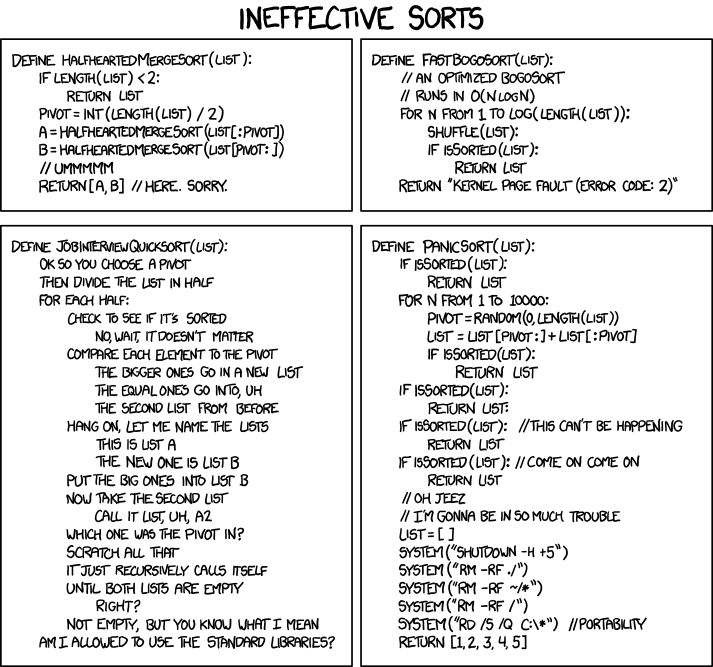
\includegraphics[width=4in]{ineffective_sorts.png}
    \caption*{StackSort connects to StackOverflow, searches for 'sort a list', and downloads and runs code snippets until the list is sorted.}
\end{figure}
\end{document}
